\section{Bigger Better Bugs}

\begin{frame}[noframenumbering, plain]
    \sectionpage    
\end{frame}

\begin{frame}{Moving Past Memory Corruption}
    \begin{columns}
        \begin{column}{0.4\textwidth}
            \begin{itemize}
                \item Vulnerabilities are much more complex than memory corruption, there needs
                to be more general systems to detect such issues.
            \end{itemize}
            \vspace{0.5cm}
            \begin{itemize}
                \item vf3 has experimental SDK support for logic bugs.
            \end{itemize}
            \vspace{0.5cm}
        \end{column}
        \begin{column}{0.6\textwidth}
            \AnimateOnly{1}{%
                \begin{figure}
                    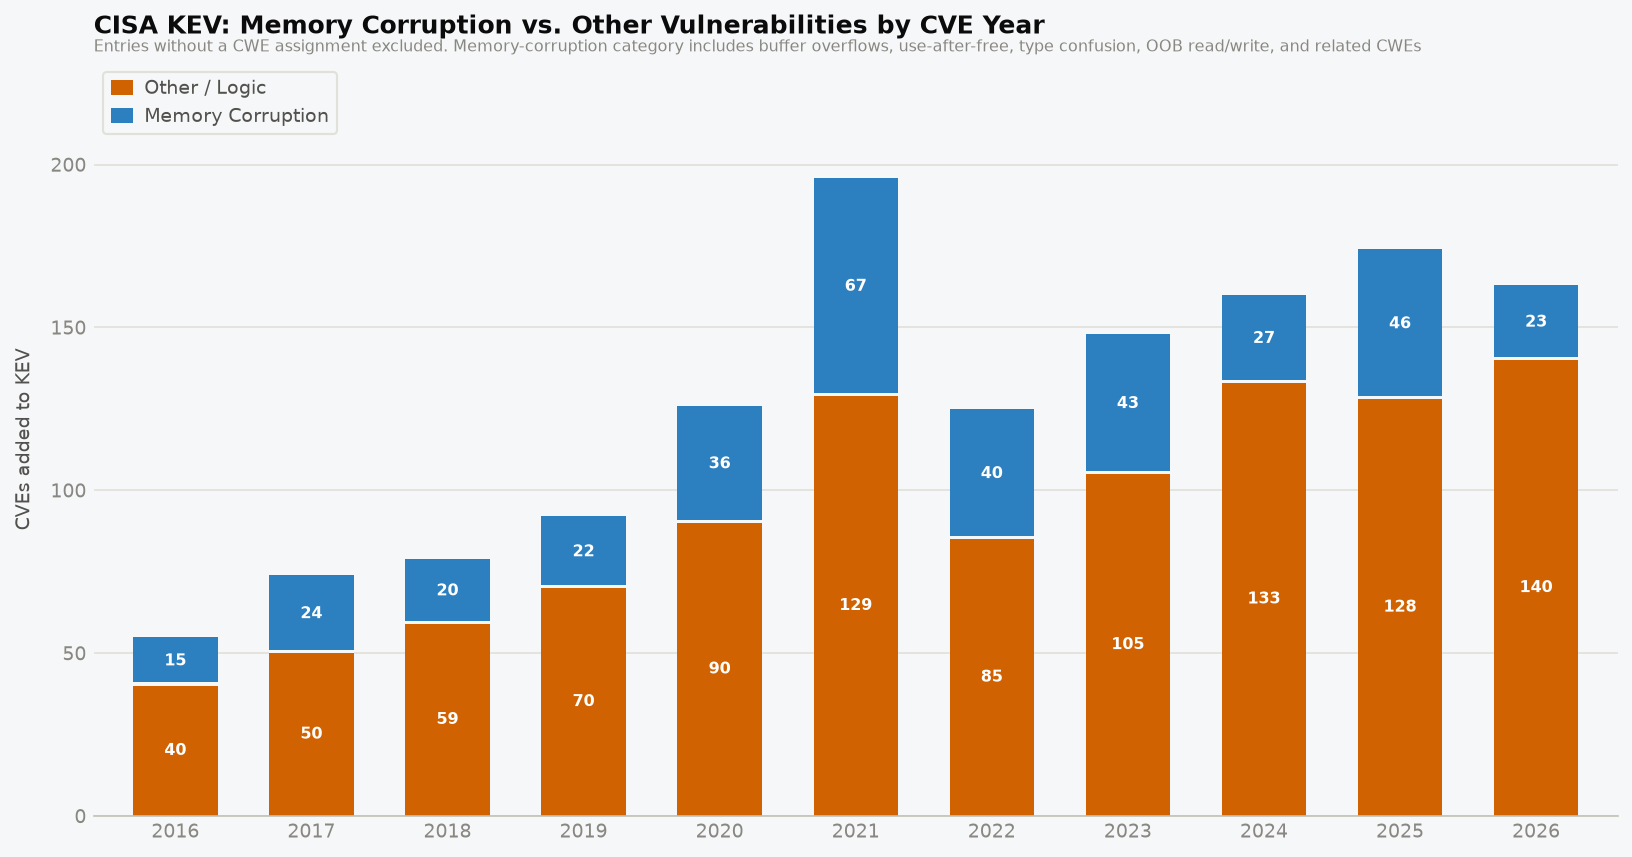
\includegraphics[width=0.95\textwidth]{images/kev_trends.png}
                    \caption{CISA KEV catalog vulnerabilities per year as memory corruption or logic issues.}
                \end{figure}
            }
            % Do not include the code snippet if animations are compiled off
            \iftoggle{ANIMATIONS}{%
                \AnimateOnly{2}{%
                    \begin{small}
                        \inputminted[style=gruvbox-dark]{python}{code/harness.py}
                    \end{small}
                }
            }{}
        \end{column}
    \end{columns}
    \vspace{-0.5cm}
\end{frame}

\begin{frame}{Cost Complexity and Tokens}
    \begin{itemize}
        \item vf3 has backwards compatibility with both AFL++ and libfuzzer harnesses.
        \item Excluding the reproducer, open-source models control the engine well.
    \end{itemize}

    \vspace{0.33cm}
    \begin{table}
        \begin{tabular}{c|c|c}
            Model & Size & Correctness (N = 100) \\
            \hline
            Granite 4-1:30b & 17G & 49\% \\
            Deepseek-r1:14b & 9G & 4\% \\
            qwen-3.8 & 17G & 90\% \\
            Sonnet 4.6 & cloud & 99\% \\
        \end{tabular}
        \caption{Performance of various models in patch gapping N-days in Apache httpd.}
    \end{table}
    \vspace{-0.25cm}
\end{frame}
